\begin{figure}[htb]
    \centering
    \begin{subfigure}[b]{0.5\floatwidth}
        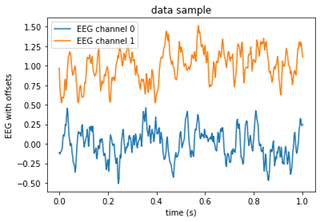
\includegraphics[width=\textwidth]{5Results/figs/samples/double_interictal_sample.png}
    \end{subfigure}
    \hfill    
    \begin{subfigure}[b]{0.5\floatwidth}
        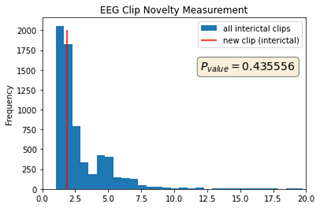
\includegraphics[width=\textwidth]{5Results/figs/samples/double_interictal_pvalue.png}
    \end{subfigure}
    \\
    \begin{subfigure}[b]{0.5\floatwidth}
        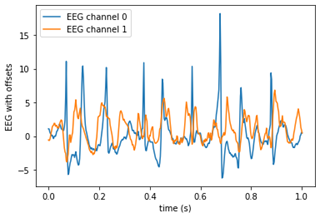
\includegraphics[width=\textwidth]{5Results/figs/samples/double_ictal_sample.png}
    \end{subfigure}
    \hfill
    \begin{subfigure}[b]{0.5\floatwidth}
        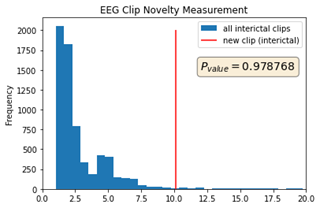
\includegraphics[width=\textwidth]{5Results/figs/samples/double_ictal_pvalue.png}
    \end{subfigure}
    \Caption{Anomaly detection}{
	An interictal double-channel segment has a p-value of 0.435 (top). An ictal double-channel segment has a p-value of 0.978 (bottom).
	\protect \NS[inline]{remake example likelihood estimation figures}
    }
    \label{fig:5results:samples}
\end{figure}
